\documentclass{article}
\usepackage[final]{nips_2018}
\usepackage[utf8]{inputenc} % allow utf-8 input
\usepackage[T1]{fontenc}    % use 8-bit T1 fonts
\usepackage{hyperref}       % hyperlinks
\usepackage{url}            % simple URL typesetting
\usepackage{booktabs}       % professional-quality tables
\usepackage{amsfonts}       % blackboard math symbols
\usepackage{nicefrac}       % compact symbols for 1/2, etc.
\usepackage{microtype}      % microtypography
\usepackage{enumerate}
\usepackage{graphicx} 
\usepackage{float} 
\title{Prediction Model on Graduate Admission}
\author{%
  Deng Yiqi\\
  Computer Science Dept. \\
  The University of Hong Kong\\
  \texttt{yqdeng@cs.hku.hk} \\
  % examples of more authors
  \And
  Kuang Mengmeng \\
  Computer Science Dept. \\
  The University of Hong Kong\\
  \texttt{mmkuang@cs.hku.hk} \\
  \And
  Yu Huijing \\
  Computer Science Dept. \\
  The University of Hong Kong\\
  \texttt{hjyu@cs.hku.hk} \\
}

\begin{document}
\maketitle
\begin{abstract}
  As the increasing number of students applying for a postgraduate degree, the admission for graduate school has been getting more and more competitive. In addition, the process to apply for graduate school is intensive and expensive. We have obtained a dataset of students’ admission information to a particular graduate school, such as GPA, GRE score, TOEFL score and so on. We propose a combined algorithm based on some popular machine learning algorithms, to improve the predicting results. With our model, students will be able to evaluate their chances of being accepted to graduate school and decide if they will apply. If applying, the model could also help them enhance and refine their application strategies.
\end{abstract}

\section{Introduction}
A rising level of pursuing higher education in general population has introduced a great competition among applicants. Therefore, both students and parents pay careful attention to the factors that will lead to a higher chance of admission. For example, for the “Gaokao” in China, the examination score is the sole factor that decides a student’s admission to the college. In other countries, there are multiple factors that could influence one’s admission to graduate school. Some obvious variables such as GPA, TOEFL score and GRE score, which directly indicate one’s learning abilities and English proficiency, are considered to be core standards by some college admission committee and have a direct impact on student’s admission. It is commonly known that the higher the GPA or TOEFL or GRE score a student can get, the bigger the chance they will be able to get an offer from a college. However, some universities might not consider score as important as we thought. They might value other implicit variables more important, such as the student’s undergraduate program ranking, statement of purpose, the strength of recommendation letter and research experience. Therefore it is hard to predict the admission chance just based on score using simple linear regression. In addition, different universities might value these variables differently. Some might consider a higher undergraduate program ranking indicates a greater possibility of success. Some might think a strong letter recommendation from a well-known professor shows a bigger chance of academic success in graduate school. Some might consider research experience during undergraduate is a good indicator of research potential and ability. Therefore, in this project, we obtain a dataset of students’ admission information to one particular graduate school. We will take a basic look at the dataset and conclude which variables are crucial for admission to this graduate school. We will take into account all the variables mentioned above and develop an admission prediction model by using Machine Learning algorithms. We could also generalize the model to work with different graduate school student admission data to compensate for the fact that different universities have different admission standards. 

\section{Method}
\subsection{Data}
To be more concrete, we obtained a dataset\textsuperscript{[1]} that includes several factors that are considered as significant during application. Those factors are:

\begin{enumerate}[1.]
	\item GRE Scores(out of 340);
	\item TOEFL Scores(out of 120);
	\item University Rating ( out of 5, higher scores for higher rank);
	\item Statement of Purpose and Letter of Recommendation Strength(out of 5, higher scores for valuable strength); 
	\item Undergraduate GPA(out of 10, higher scores for higher GPA);  
	\item Research Experience(either 0 or 1). 
\end{enumerate}

\subsection{Algorithm}
Common regression algorithm includes Linear Regression, Random Forest Regression, Decision Tree Regression and so on. There are also some conventional classification algorithms, such as logistic regression, SVM, Decision Tree Classification, GDBT, XGBoost, and etc. For a very similar problem like house price prediction\textsuperscript{[2]}, where multiple variables are being taken into account, the author used the algorithms called Least Absolute Shrinkage and Selection Operator (Lasso), and XGBoost. Combined with the use of ElasticNet, they had a relatively desirable performance result\textsuperscript{[3]}. Therefore, in our project, we are planning to develop a model combined with some existing algorithms, with further enhancement and modification in order to reach a better performance and more accurate results.

	The overall algorithm has two layers:
	\begin{enumerate}[1.]
	\item Through classification algorithms, the data will be divided into two groups based on its chance of admission (0-50\ \%, 50\ \%-100\ \%). Then each group of data will be normalized separately.
	\item We will use various regression algorithms to perform fitting on each group of the data separately. 
	\end{enumerate}
	
Lastly, some of the outputs from layer two will be handled through certain weight distribution and generate a final result (just like how it is handled in the house price prediction problem\textsuperscript{[2]}).

The flowchart is described as Figure 1: 

\begin{figure}[H] 
\centering 
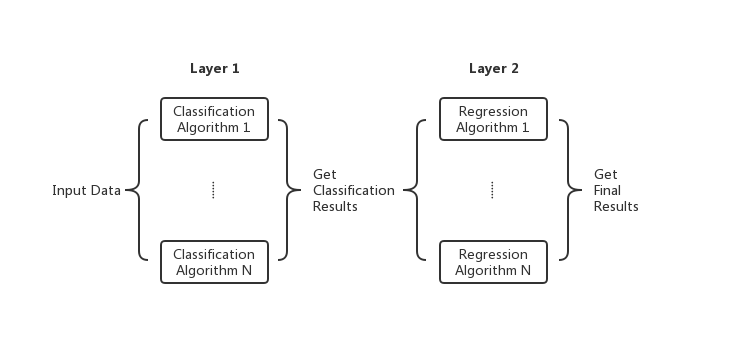
\includegraphics[width=0.7\textwidth]{layers} 
\caption{Flowchart of Our Algorithm} 
\label{Flowchart of Our Algorithm} 
\end{figure}

\section{Evaluation}
Our proposed algorithm has two layers, the first layer mainly focusing on the classification algorithm and the second layer focusing on the regression algorithms. Therefore, there are also two parts of the evaluation. The evaluation for the first layer will be only used to help us improve our proposed algorithms. The evaluation for the second layer will be our proposed algorithm’s final accuracy result. 

For the evaluation in the first layer (classification), we will use some industrialized-standard methods, such as accuracy, recall rate, and F-measure\textsuperscript{[4]}. 

Please see the following Table 1 for corresponding formulas:
\begin{table}[H]
  \caption{Precision, Recall \ \& F-measure}
  \label{Precision, Recall and F-measure}
  \centering
  \begin{tabular}{lll}
    \toprule
    \cmidrule(r){1-2}
    Name     & Formula\\
    \midrule
    Precision(P) & TP/(TP + FP)     \\
    Recall(R)     & TP/(TP + FN) \\
    F-measure(F)     & 2PR/(P + R)\\
    \bottomrule
  \end{tabular}
\end{table}

Where:
	\begin{enumerate}[-]
	\item TP: True Positives
	\item FP: False Positives
	\item FN: False Negaties
	\end{enumerate}

For the evaluation in the second layer (regression), we will utilize the coefficient of determination\textsuperscript{[5]} (R\textsuperscript{2} score).

Please see the following Table 2 for corresponding formulas:
\begin{table}[H]
  \caption{Coefficient of Determination}
  \label{Coefficient of Determination}
  \centering
  \begin{tabular}{lll}
    \toprule
    \cmidrule(r){1-2}
    Name     & Formula\\
    \midrule
    Total sum of squares & $SS_{ \mathrm{tot}}=\sum_{i}\left(y_{i}-\overline{y}\right)^{2}$     \\
    Explained sum of squares     & $S S _ { \mathrm { reg } } = \sum _ { i } \left( f _ { i } - \overline { y } \right) ^ { 2 }$ \\
    Residual sum of squares     & $S S _ { \mathrm { res } } = \sum _ { i } \left( y _ { i } - f _ { i } \right) ^ { 2 } = \sum _ { i } e _ { i } ^ { 2 }$\\
     \midrule
    The coefficient of determination & $R ^ { 2 } \equiv 1 - \frac { S S _ { \mathrm { res } } } { S S _ { \mathrm { tot } } }$ \\
    \bottomrule
  \end{tabular}
\end{table}

\section*{References}
\small
[1] Mohan S Acharya, Asfia Armaan \ \& Aneeta S Antony 
A Comparison of Regression Models for Prediction of Graduate Admissions. {\it IEEE International Conference on Computational Intelligence in Data Science 2019}

[2] House Prices: Advanced Regression Techniques: https://www.kaggle.com/c/house-prices-advanced-regression-techniques

[3] HousePrices GitHub Code: https://github.com/kuangmeng/HousePrices

[4] Davis, Jesse Goadrich \ \& Mark 
The Relationship Between Precision-Recall and ROC Curves. {\it ICML '06, ACM} (P. 233 -- 240)

[5] Coefficient of Determination: https://dwz.cn/nBMdGC8i

\end{document}